\documentclass[final]{beamer}
\usepackage[scale=1.24]{beamerposter}

\usetheme{confposter}

% ── Poster dimensions ─────────────────────────────────────
\newlength{\sepwid}
\newlength{\onecolwid}
\newlength{\twocolwid}
\newlength{\threecolwid}
\setlength{\paperwidth}{80in}
\setlength{\paperheight}{40in}
\setlength{\sepwid}{0.024\paperwidth}
\newlength{\colA}\setlength{\colA}{0.31\paperwidth}   % Col 1: Motivation + Method
\newlength{\colB}\setlength{\colB}{0.29\paperwidth}   % Col 2: Framework + Theory
\newlength{\colC}\setlength{\colC}{0.26\paperwidth}   % Col 3: Experiments (narrower)
\setlength{\onecolwid}{0.3\paperwidth}
\setlength{\twocolwid}{0.625\paperwidth}
\setlength{\threecolwid}{0.904\paperwidth}
\setlength{\topmargin}{-0.5in}

% ── Packages ──────────────────────────────────────────────
\usepackage{graphicx}
\usepackage{booktabs}
\usepackage{amsmath,amssymb,amsfonts}
\usepackage[T1]{fontenc}
\usepackage{microtype}
\usepackage{tcolorbox}
\tcbuselibrary{skins}
\usepackage{multicol}
\usepackage{enumitem}
\usepackage{wrapfig}

% ── Colors (override confposter defaults) ─────────────────
\definecolor{samsungblue}{HTML}{1428A0}
\definecolor{samsunglight}{HTML}{E8EAF6}
\definecolor{accentgreen}{HTML}{2E7D32}
\definecolor{darktext}{HTML}{212121}
\definecolor{theorybg}{HTML}{FFF8E1}
\definecolor{resultbg}{HTML}{E8F5E9}
\definecolor{sectionbg}{HTML}{F0F4FF}
\definecolor{golden}{RGB}{255,200,0}
\definecolor{turquoise}{RGB}{72,209,204}

% Override block colors for Samsung style
\setbeamercolor{block title}{fg=samsungblue,bg=white}
\setbeamercolor{block body}{fg=darktext,bg=white}
\setbeamercolor{block alerted title}{fg=white,bg=turquoise!60!white}
\setbeamercolor{block alerted body}{fg=black,bg=turquoise!15!white}
\setbeamercolor{title in headline}{fg=samsungblue}
\setbeamercolor{separation line}{bg=samsungblue}

% ── Math ──────────────────────────────────────────────────
\newcommand{\Hsim}{H_{\mathrm{sim}}}
\newcommand{\bx}{\mathbf{x}}

% ══════════════════════════════════════════════════════════
\title{Query-Aware Flow Diffusion for Graph-Based RAG with Retrieval Guarantees}

\author{%
  Zhuoping Zhou$^{*}$ \quad
  Davoud Ataee Tarzanagh$^{*}$ \quad
  Sima Didari$^{*}$ \quad
  Wenjun Hu \quad
  Baruch Gutow \quad
  Oxana Verkholyak \quad
  Masoud Faraki \quad
  Heng Hao \quad
  Hankyu Moon \quad
  Seungjai Min%
}

\institute{Samsung SDS Research America, Mountain View, CA, USA \hspace{3em} $^{*}$Equal contribution}

% ══════════════════════════════════════════════════════════
\begin{document}

\addtobeamertemplate{block end}{}{\vspace*{2ex}}
\addtobeamertemplate{block alerted end}{}{\vspace*{2ex}}
\setlength{\belowcaptionskip}{2ex}
\setlength\belowdisplayshortskip{2ex}

\begin{frame}[t]

% ICLR logo in top-left corner
\begin{tikzpicture}[remember picture,overlay]
  \node[anchor=north west, inner sep=0pt] at ([xshift=1.5cm, yshift=-1.5cm]current page.north west)
    {
\includegraphics[height=5cm]{figs/iclr_logo.png}};
\end{tikzpicture}
% Samsung SDS logo in top-right corner
\begin{tikzpicture}[remember picture,overlay]
  \node[anchor=north east, inner sep=0pt] at ([xshift=-1.5cm, yshift=-1.5cm]current page.north east)
    {
\includegraphics[height=4cm]{figs/samsung_sds_logo.png}};
\end{tikzpicture}

\begin{columns}[t]

\begin{column}{\sepwid}\end{column}

% ══════════════════════════════════════════════════════════
% COLUMN 1: Motivation + Method
% ══════════════════════════════════════════════════════════
\begin{column}{\colA}

\vspace{-1cm}

\begin{block}{\Large\textbf{\color{samsungblue} Motivation \& Contributions}}

Graph-based RAG captures multi-hop relationships that flat retrieval misses, but existing methods rely on heuristic subgraph selection with no guarantees:

\vspace{0.3em}
\colorbox{samsunglight}{\parbox{0.95\linewidth}{%
  $\bullet$ \textbf{GraphRAG:} Static community detection --- mixes relevant and irrelevant nodes\\[3pt]
  $\bullet$ \textbf{LightRAG:} 1-hop ego-networks --- misses global context\\[3pt]
  $\bullet$ \textbf{Both:} No guarantees on completeness or precision of retrieved subgraphs
}}

\vspace{0.3em}
\begin{center}
  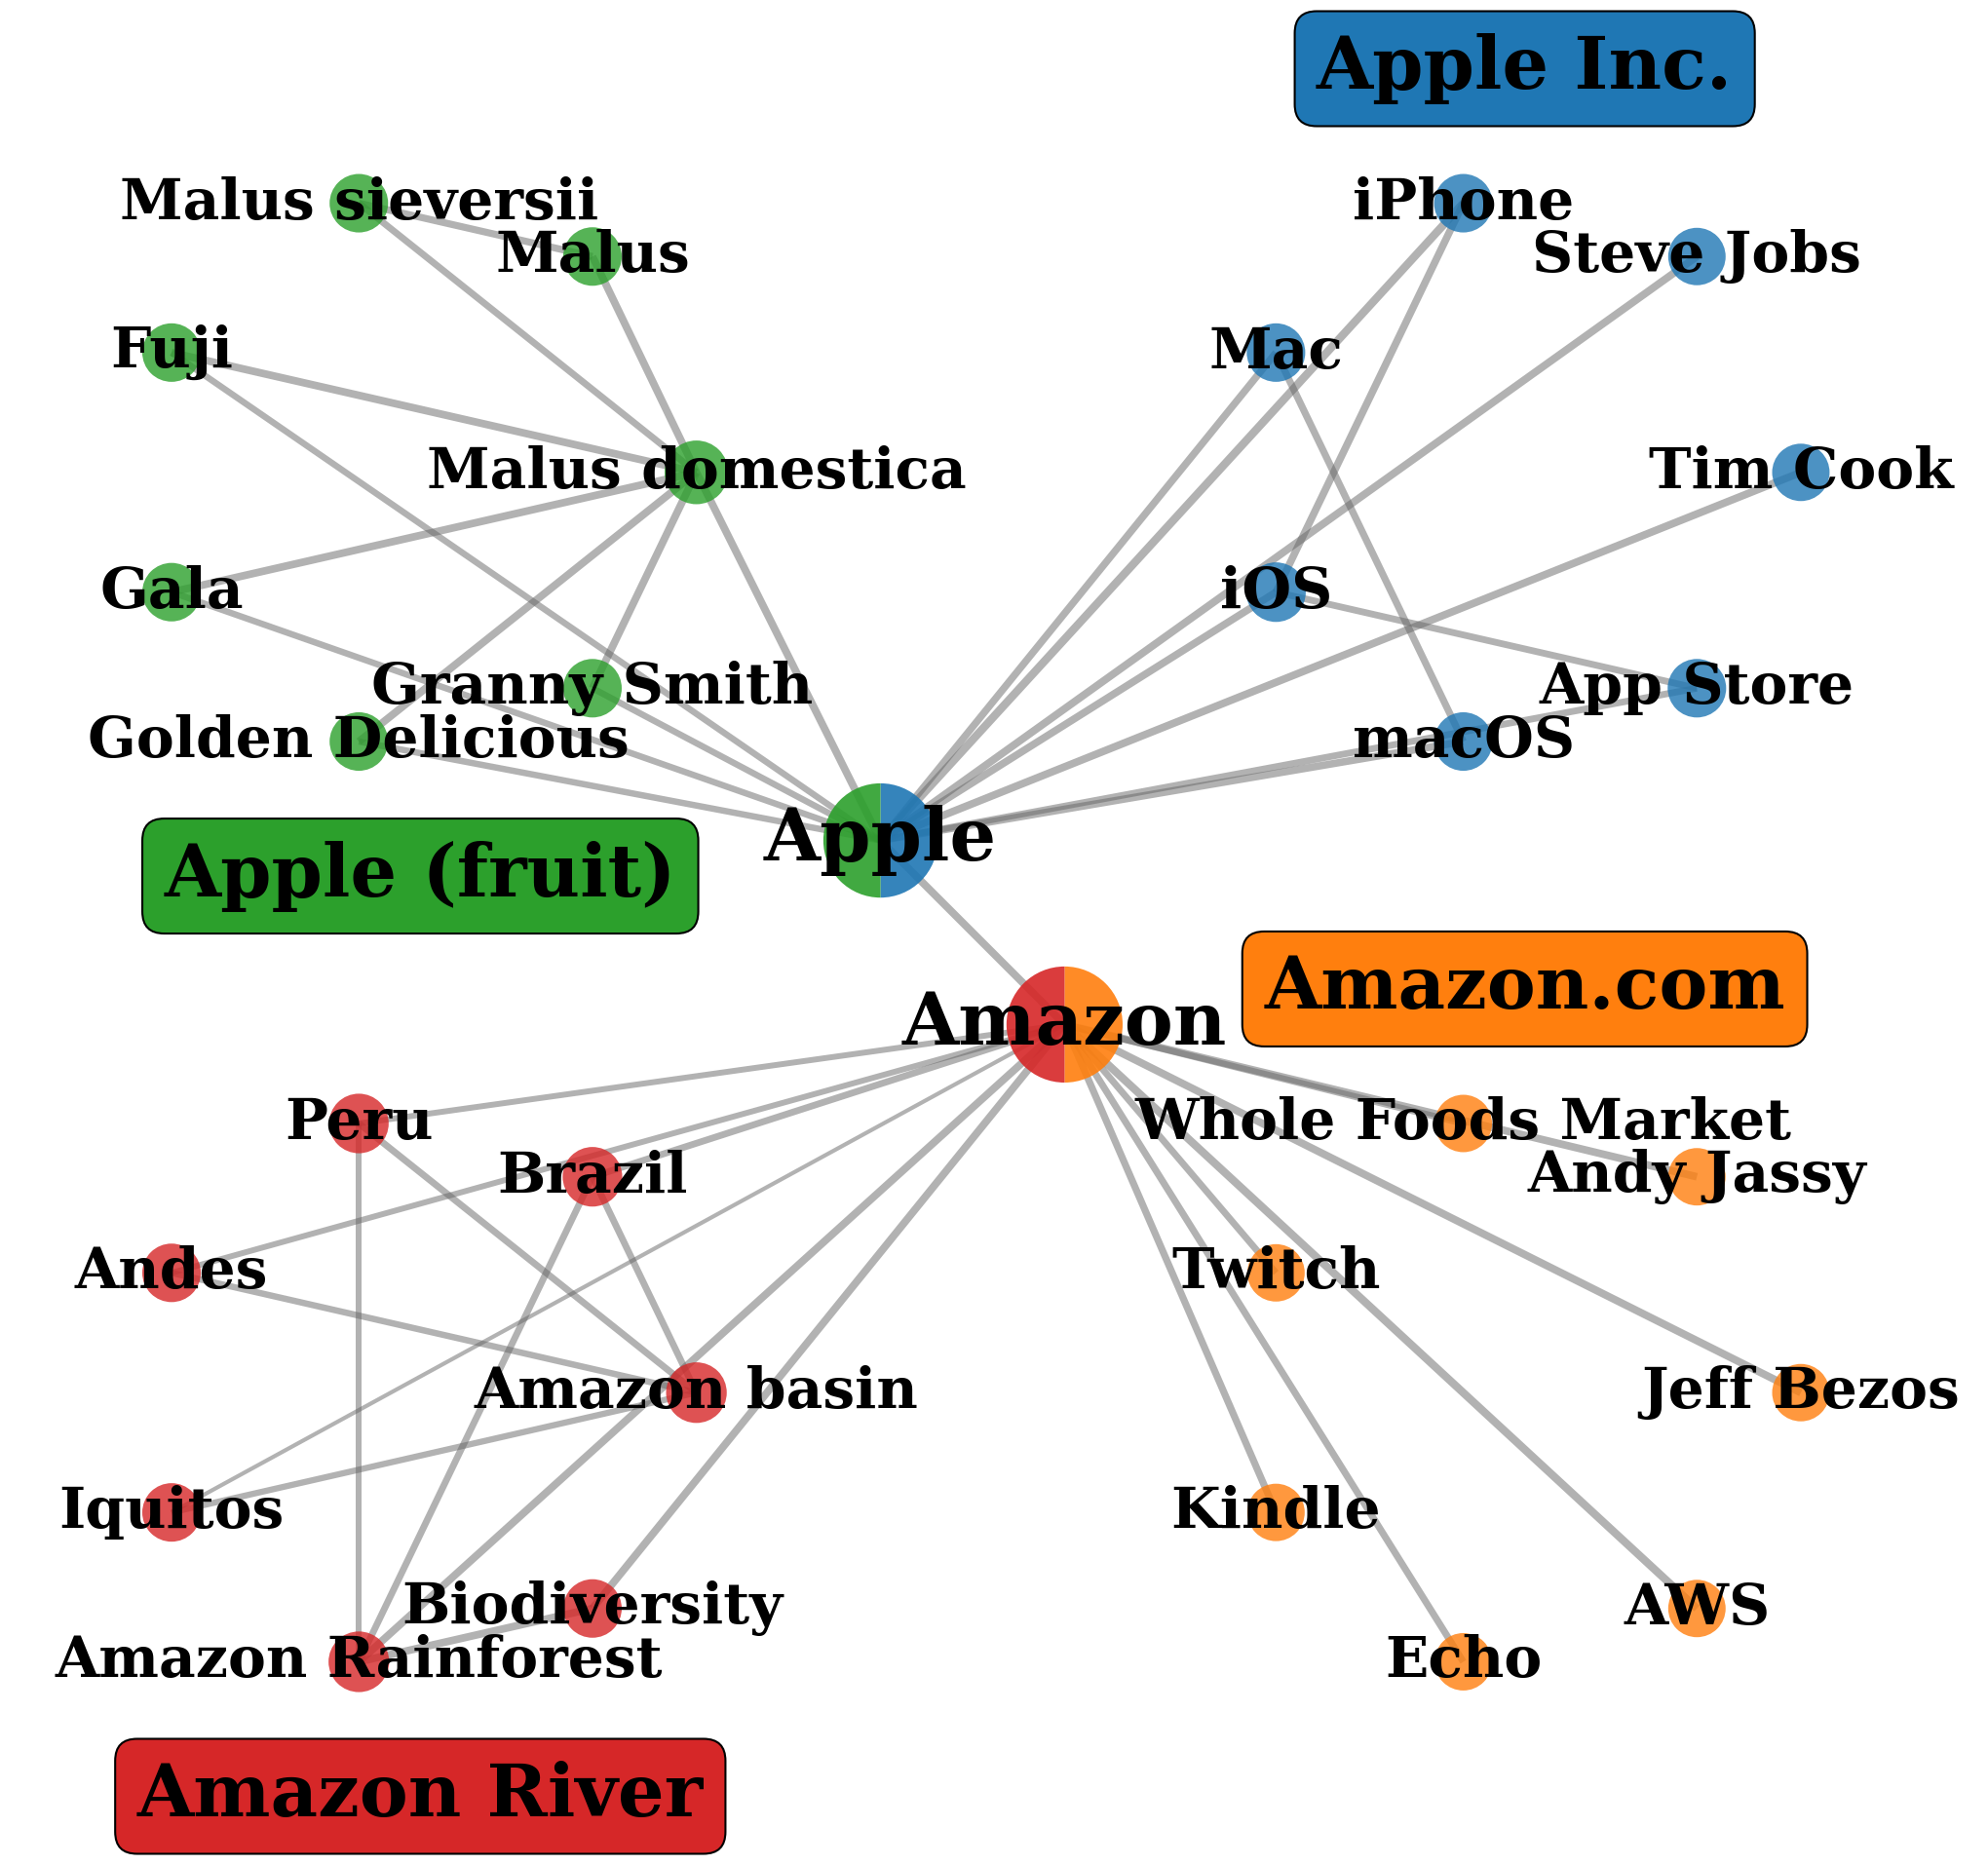
\includegraphics[height=10cm]{figs/GraphRAG.png}\hspace{0.3em}%
  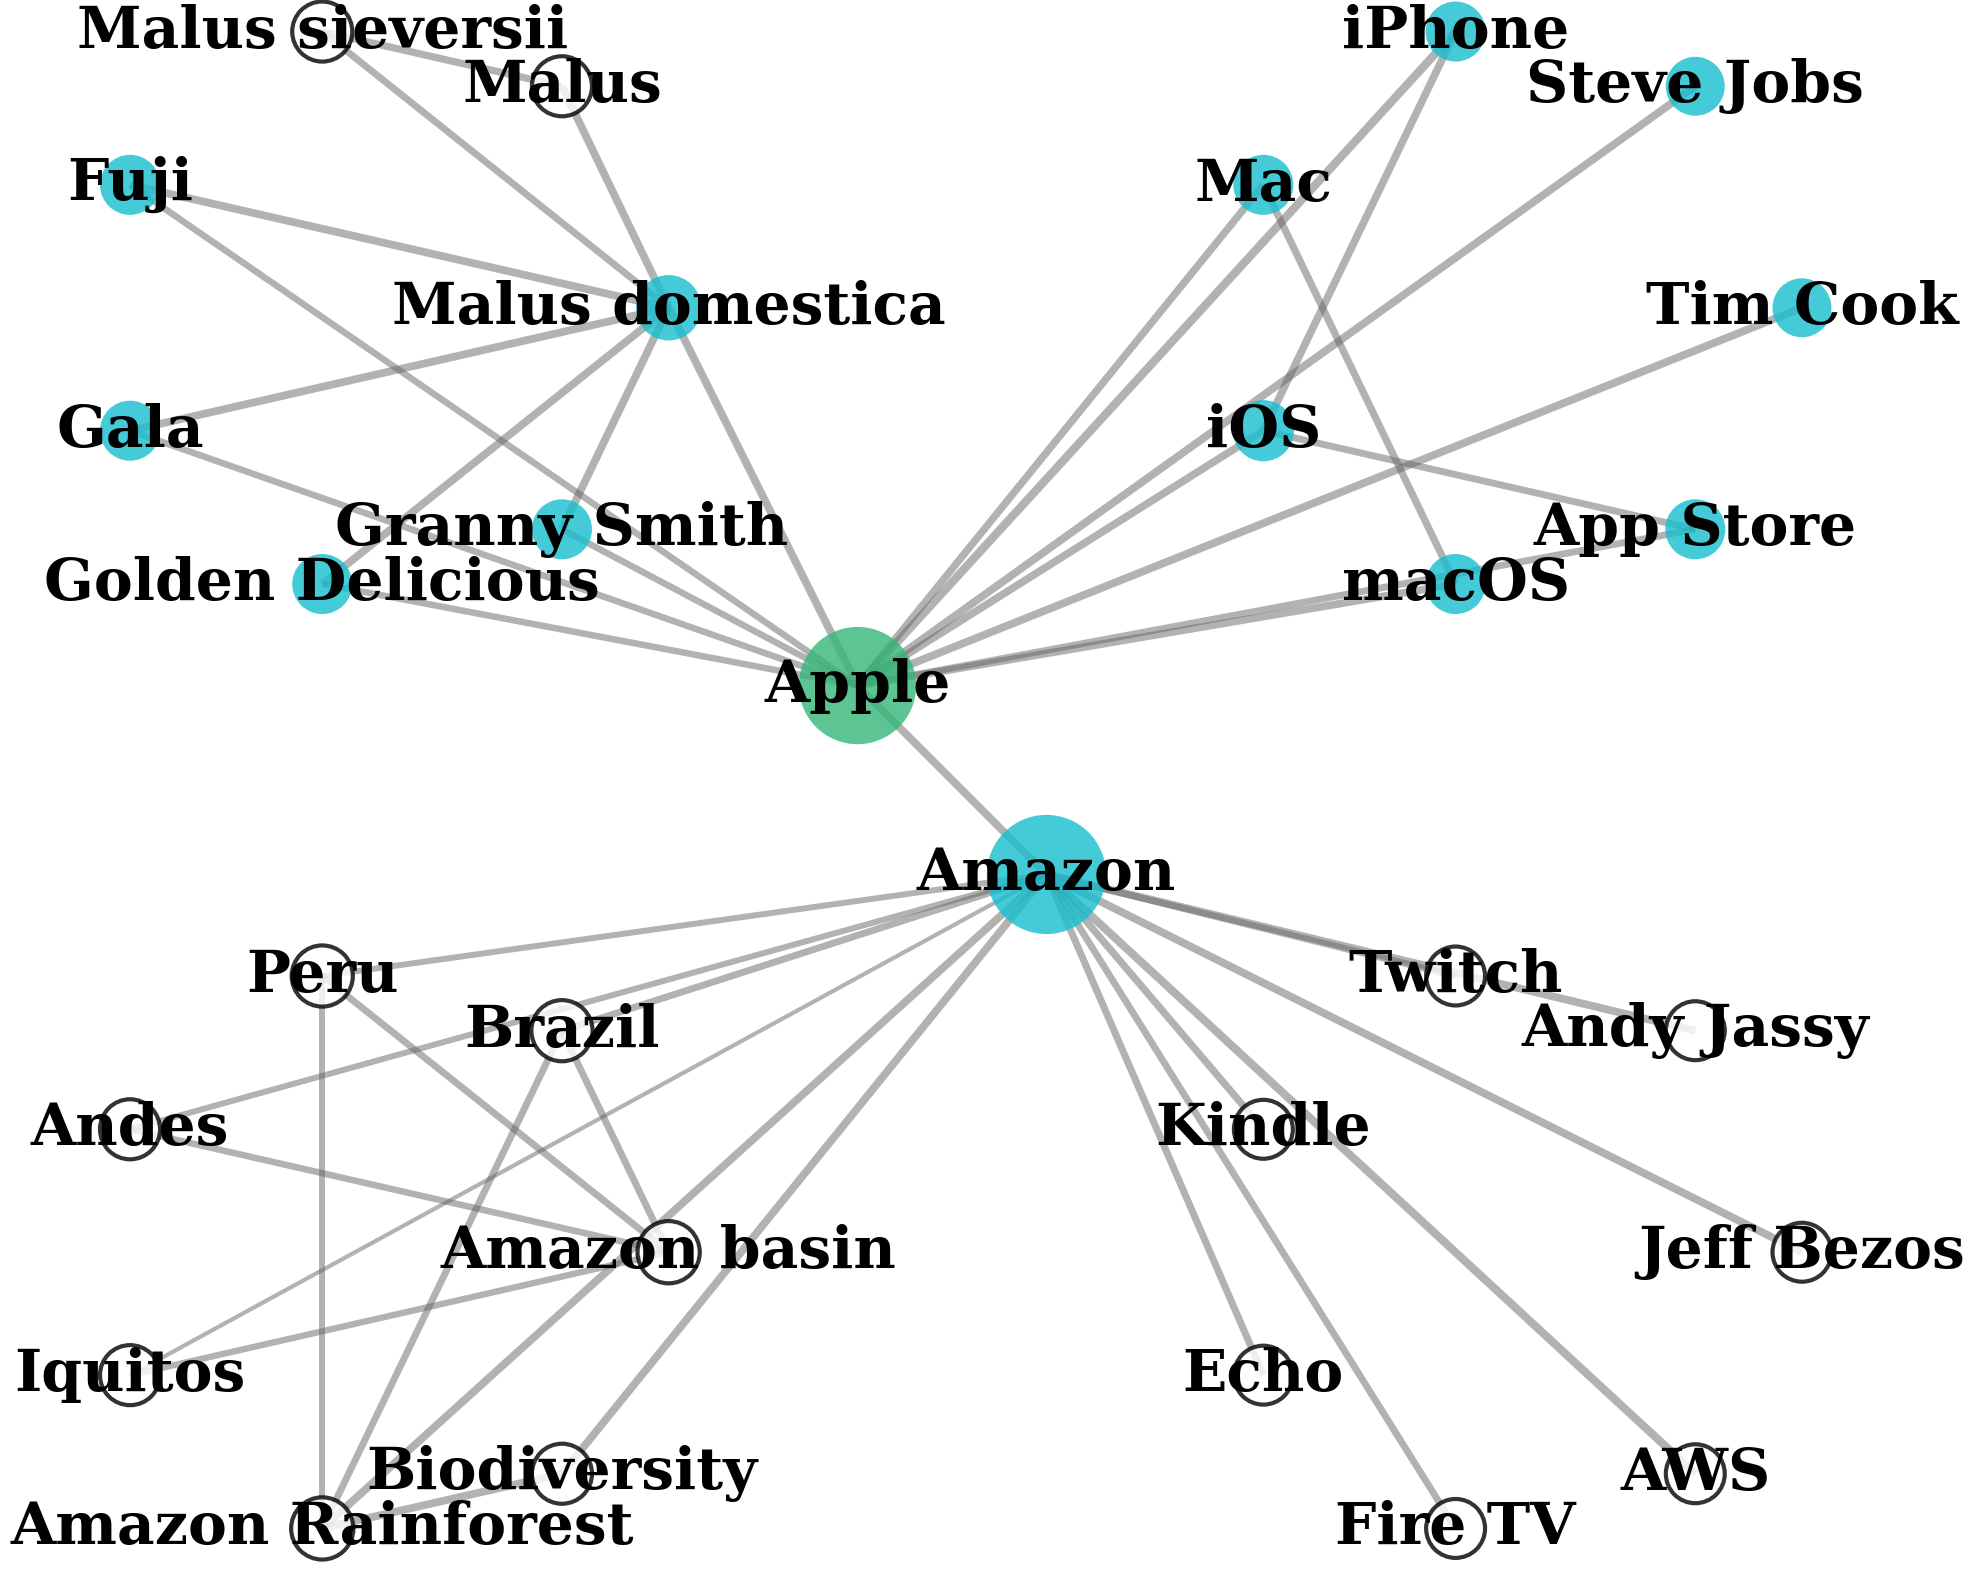
\includegraphics[height=10cm]{figs/LightRAG.png}\hspace{0.3em}%
  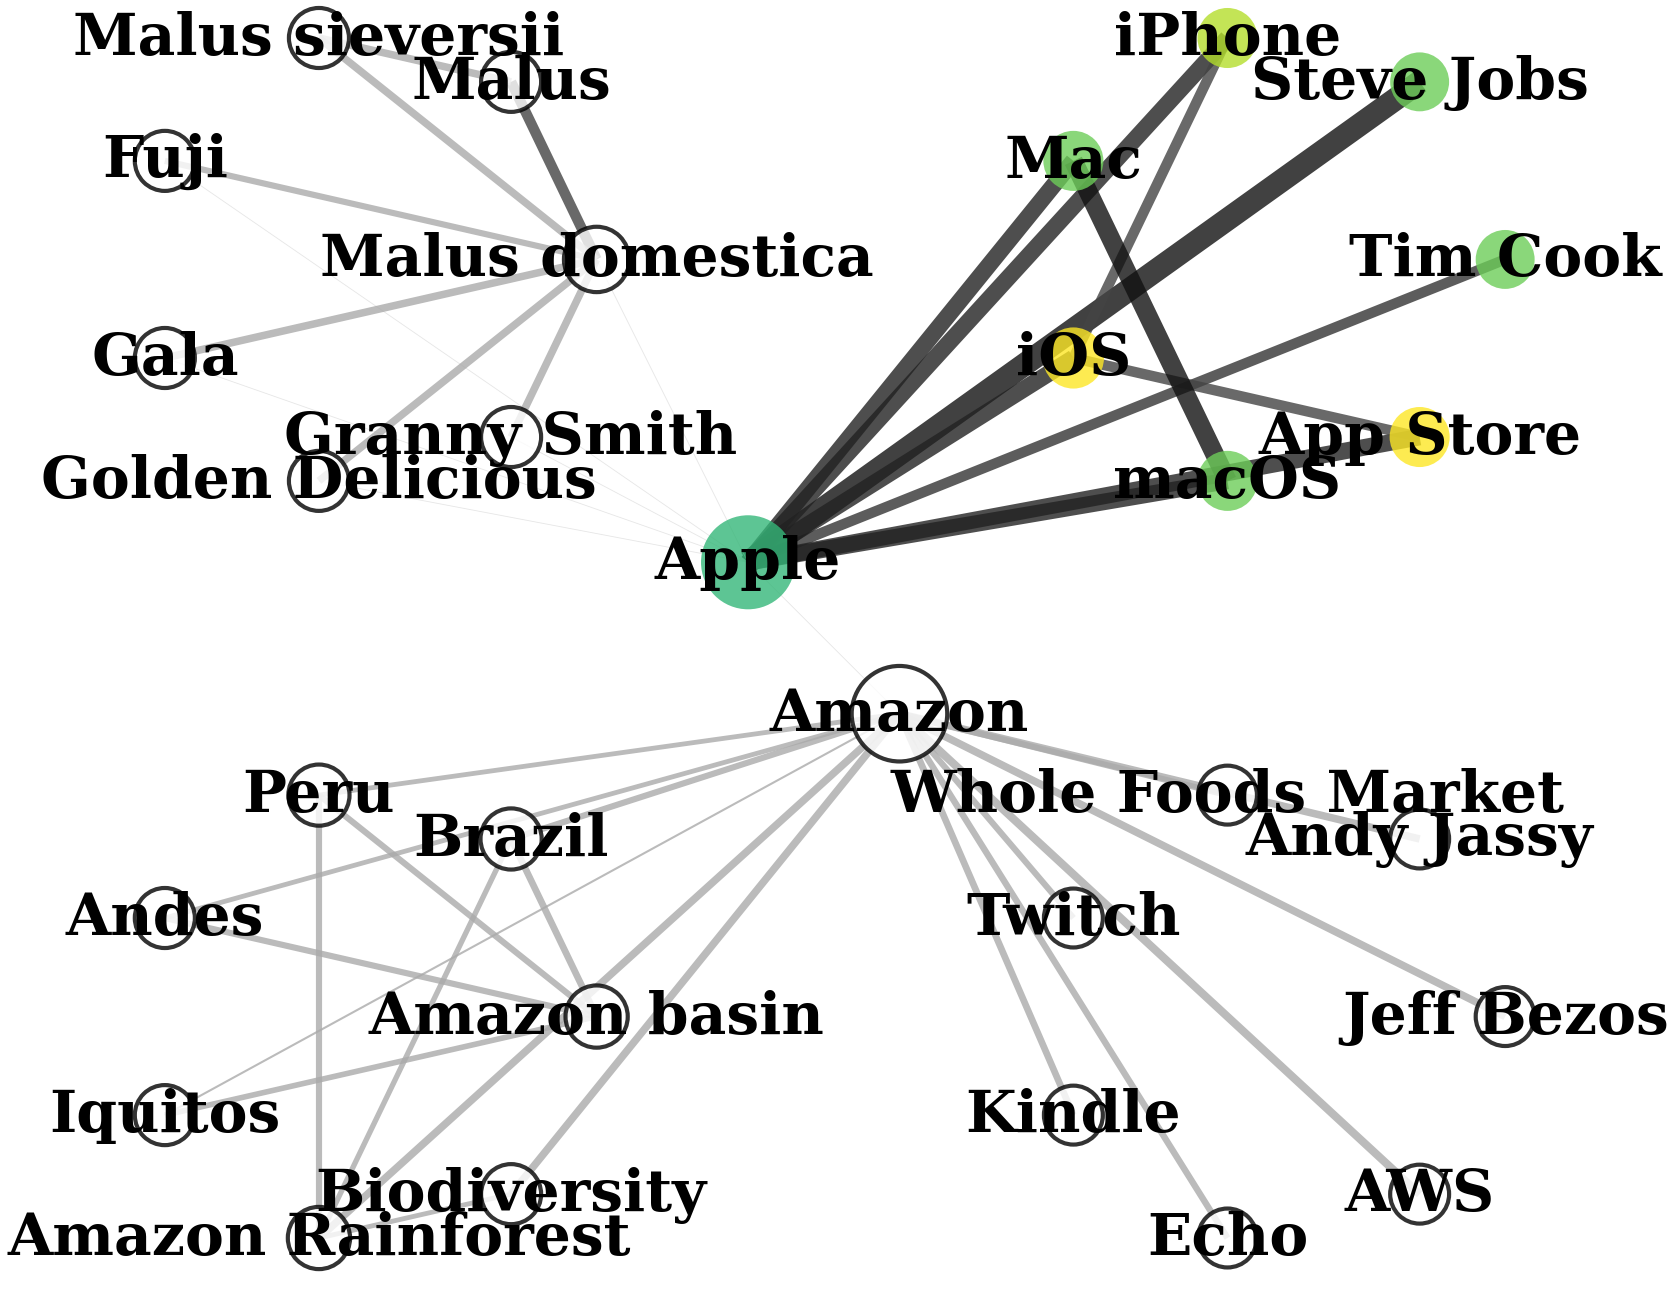
\includegraphics[height=10cm]{figs/QAFD-RAG.png}
\end{center}
\vspace{-0.3em}
\begin{center}
  \small\textit{Query: ``Introduce Steve Jobs's products in Apple.''}\\[2pt]
  \textbf{GraphRAG} (communities) \;\; \textbf{LightRAG} (ego-net) \;\; \textbf{QAFD-RAG} (flow diffusion)
\end{center}

\vspace{0.3em}
\colorbox{sectionbg}{\parbox{0.95\linewidth}{%
  \textbf{Our Contributions:}\\[3pt]
  \textbf{C1.} \textbf{Query-Aware Flow Diffusion} --- the first principled flow-based retrieval for graph RAG. Edge weights adapt dynamically to each query. Runtime scales with the \emph{retrieved subgraph}, not the full graph.\\[3pt]
  \textbf{C2.} \textbf{Provable Guarantees} --- exponential convergence of the push--relabel solver (Thm.~1) and statistical recovery guarantees ensuring completeness with bounded leakage (Thm.~2).\\[3pt]
  \textbf{C3.} \textbf{State-of-the-Art Results} --- consistent gains across multi-hop QA, long-document summarization, general domain QA, and text-to-SQL benchmarks.
}}

\end{block}


\begin{block}{\Large\textbf{\color{samsungblue} Method}}

\textbf{Step 1: Seed Node Selection.}\;
Given query $q$, extract keywords $\{w_1,\ldots,w_{|K_q|}\}$ via LLM. Top-$N$ nodes by keyword similarity serve as flow sources:
$S_V = \mathrm{Top}\text{-}N_v\;\max_{i}\;\Hsim\!\bigl(h(w_i),\, h(v)\bigr)$.

\vspace{0.3em}
\textbf{Step 2: Query-Aware Edge Weighting.}\;
Edges are reweighted dynamically per query. Three variants:

\vspace{0.2em}
\begin{tcolorbox}[colback=samsunglight, colframe=samsungblue, boxrule=1.5pt, arc=3pt, top=3pt, bottom=3pt]
  \textbf{Mean:}\; $\bar{w}_{\mathrm{M}} = \tfrac{1}{3}\bigl(\Hsim(h(u),h(v)) + \Hsim(h(u),h(q)) + \Hsim(h(v),h(q))\bigr)$\\[3pt]
  \textbf{Product:}\; $\bar{w}_{\mathrm{P}} = \Hsim(h(u),h(v)) \cdot \Hsim(h(u),h(q)) \cdot \Hsim(h(v),h(q))$\\[3pt]
  \textbf{Hybrid} (best):\; $\bar{w}_{\mathrm{H}} = \Hsim(h(u),h(v)) \cdot \bigl[1 + \tfrac{1}{4}(\Hsim(h(u),h(q)) + \Hsim(h(v),h(q)))\bigr]$
\end{tcolorbox}

\vspace{0.3em}
\textbf{Step 3: Primal--Dual Flow Optimization.}\;
The \textbf{primal} minimizes flow energy subject to capacity constraints:
$\min_{\mathbf{f}\in\mathbb{R}^{|E|}}\; \tfrac{1}{2}\,\mathbf{f}^\top \mathbf{W}(q)\,\mathbf{f} \;\; \text{s.t.}\; \boldsymbol{\Delta} + \mathbf{B}\,\mathbf{W}(q)\,\mathbf{f} \leq \mathbf{T}$.
The \textbf{dual} yields a closed-form objective over node scores:
$$\min_{\bx \geq 0}\; \underbrace{\tfrac{1}{2}\,\bx^\top \mathbf{L}(q)\,\bx}_{\text{graph smoothness}} + \underbrace{\bx^\top(\mathbf{T} - \boldsymbol{\Delta})}_{\text{source/sink balance}}$$

\vspace{-0.3em}
where $\mathbf{L}(q) = \mathbf{B}\,\mathbf{W}(q)\,\mathbf{B}^\top$ is the query-aware Laplacian.

\vspace{0.3em}
\textbf{Step 4: Push--Relabel Solver.}\;
Coordinate-wise updates that only touch nodes with excess mass:

\vspace{0.2em}
\colorbox{samsunglight}{\parbox{0.95\linewidth}{%
  \textbf{1.} Inject mass $m_s = \alpha \sum_v T_v$ at seed $s$; init $\bx = \mathbf{0}$\\[2pt]
  \textbf{2.} Pick node $v$ with excess mass ($m_v > T_v$)\\[2pt]
  \textbf{3.} Compute $\bar{w}(q,v,u)$ lazily (on-demand) for neighbors\\[2pt]
  \textbf{4.} Push excess to neighbors; update $x_v$\\[2pt]
  \textbf{5.} Repeat until $\sum_v \max(0, m_v - T_v) \leq \varepsilon$
}}

\vspace{0.2em}
Runtime is \textbf{sublinear in $|V|$} --- flow only reaches a local neighborhood.

\vspace{0.3em}
\textbf{Multi-hop:}\;
LLM decomposes $q$ into subqueries $\{q_1,\ldots,q_K\}$; final context: $G_q = \bigcup_{k=1}^K G_{q_k}$.

\end{block}

\end{column}

\begin{column}{\sepwid}\end{column}

% ══════════════════════════════════════════════════════════
% COLUMN 2: Framework Overview + Theory
% ══════════════════════════════════════════════════════════
\begin{column}{\colB}

\vspace{-1cm}

\begin{block}{\Large\textbf{\color{samsungblue} Framework Overview}}

\textbf{Indexing:} Extract entities and relations from documents to build a knowledge graph with node embeddings.
\textbf{Query:} Extract keywords, select seeds, run flow diffusion, and prompt the LLM with retrieved context.

\vspace{0.3em}
\begin{center}
  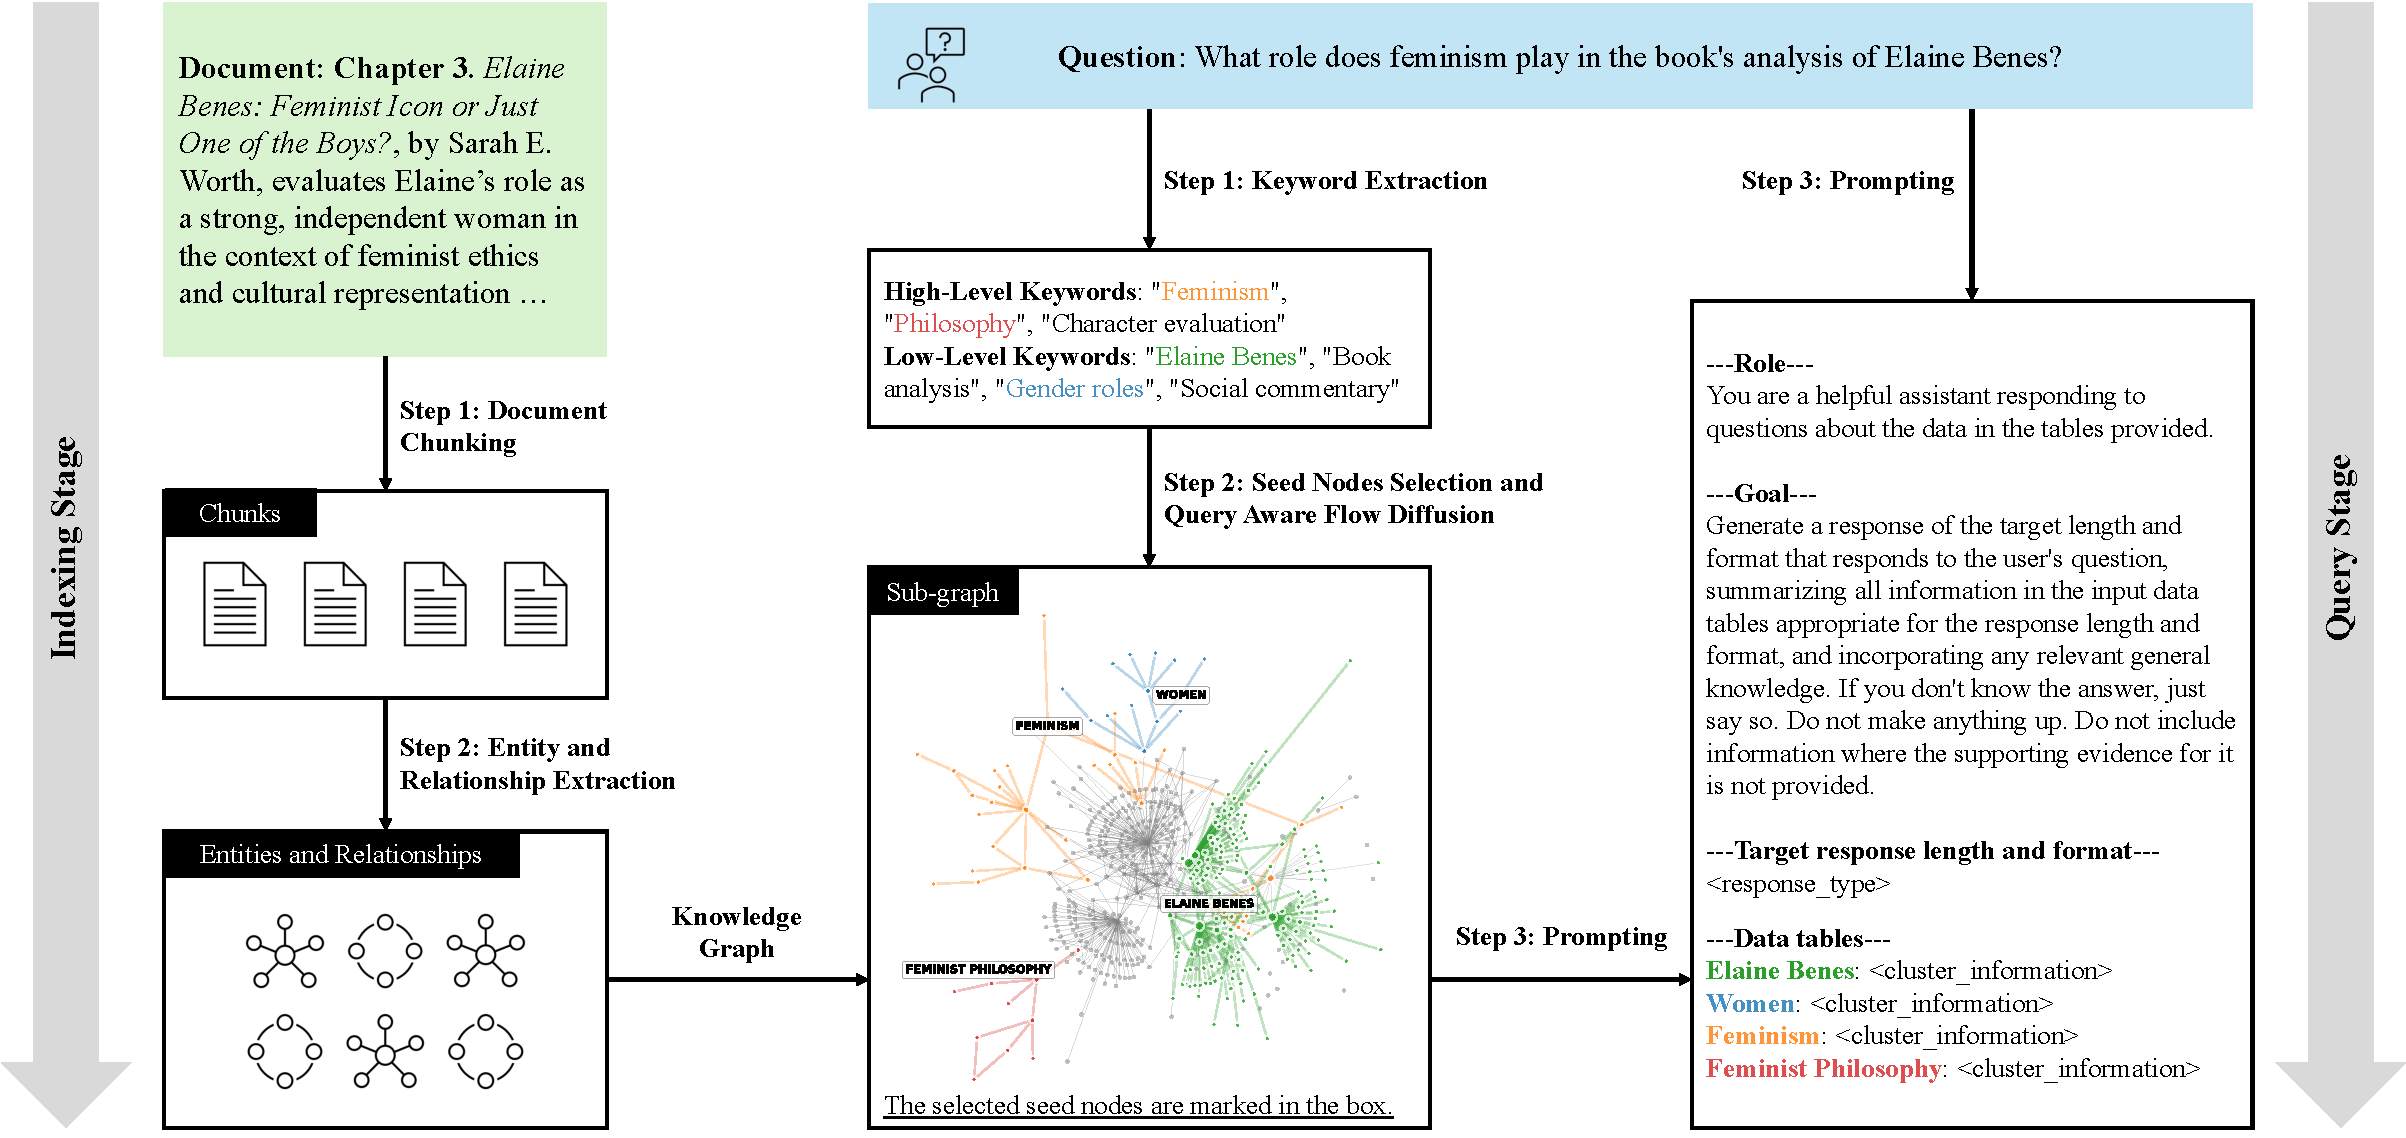
\includegraphics[width=1.0\linewidth]{figs/question_illustration.pdf}
\end{center}
\vspace{-0.3em}
\begin{center}
  \small\textit{Left: Indexing stage.\quad Right: Query processing with flow diffusion.}
\end{center}

\end{block}


\begin{alertblock}{\Large\textbf{Theorem 1 (Convergence)}}

The push--relabel algorithm converges \textbf{exponentially fast}:
$$\tau = \mathcal{O}\!\Bigl(\|\boldsymbol{\Delta}\|_1 \cdot \frac{\gamma}{\eta} \cdot \log \frac{1}{\xi}\Bigr) \text{ iterations}$$

where $\gamma$ = max weighted degree, $\eta$ = min edge weight in optimal support, $\xi$ = tolerance. Bound depends on \emph{local} support, not full graph size.

\end{alertblock}


\begin{alertblock}{\Large\textbf{Theorem 2 (Recovery Guarantee)}}

Under signal-to-noise condition $\hat{\mu}/\hat{\sigma} = \omega(\sqrt{d\log|V|})$, flow diffusion recovers relevant nodes w.h.p.:

\vspace{0.5em}
$\bullet$ \textbf{Completeness:} $R_k \subseteq \mathrm{support}(\bx^*)$ \hfill {\small(all relevant nodes recovered)}

\vspace{0.3em}
$\bullet$ \textbf{Bounded leakage:} $\displaystyle\sum_{u \notin R_k} T_u \leq \beta \sum_{u \in R_k} T_u$ \hfill {\small($\beta$ controls precision)}

\vspace{0.3em}
$\beta$ controls precision--recall trade-off: smaller $\beta$ yields tighter subgraphs.

\end{alertblock}


\begin{block}{\Large\textbf{\color{samsungblue} Key Properties}}

\colorbox{sectionbg}{\parbox{0.95\linewidth}{%
$\bullet$ \textbf{Sublinear complexity:} Runtime scales with retrieved subgraph, not full graph.\\[5pt]
$\bullet$ \textbf{Lazy evaluation:} Edge weights computed on-demand as flow propagates.\\[5pt]
$\bullet$ \textbf{First provable guarantees} for query-aware graph retrieval in RAG.\\[5pt]
$\bullet$ \textbf{Multi-hop:} Subquery decomposition with merged contexts: $G_q = \bigcup_{k} G_{q_k}$.
}}

\end{block}

\end{column}

\begin{column}{\sepwid}\end{column}

% ══════════════════════════════════════════════════════════
% COLUMN 3: Experimental Results
% ══════════════════════════════════════════════════════════
\begin{column}{\colC}

\vspace{-1cm}

\begin{block}{\Large\textbf{\color{samsungblue} Experimental Results}}

\setlength{\intextsep}{0pt}
\setlength{\columnsep}{1em}

% ── Multi-Hop QA ──────────────────────────────────────────
\textbf{\large\color{samsungblue} Multi-Hop QA}\par\vspace{0.3em}
\begin{wraptable}{r}{0.60\linewidth}
\vspace{-0.8em}
\scriptsize
\begin{tabular}{l cc cc cc}
  \toprule
  & \multicolumn{2}{c}{\textbf{HotpotQA}} & \multicolumn{2}{c}{\textbf{2Wiki}} & \multicolumn{2}{c}{\textbf{MuSiQue}} \\
  \cmidrule(lr){2-3} \cmidrule(lr){4-5} \cmidrule(lr){6-7}
  & F1 & EM & F1 & EM & F1 & EM \\
  \midrule
  GraphRAG  & 33.4 & 14.0 & 15.2 & 7.0  & 39.4 & 17.6 \\
  LightRAG  & 8.8  & 0.0  & 8.2  & 1.0  & 1.4  & 0.1  \\
  RAPTOR    & 52.3 & 25.0 & 38.8 & 12.0 & 28.1 & 10.5 \\
  HippoRAG & 58.7 & 45.3 & \textbf{70.3} & \textbf{61.2} & 38.3 & 27.6 \\
  \midrule
  \textbf{QAFD} & \textbf{73.4} & \textbf{58.1} & 69.4 & 59.5 & \textbf{48.0} & \textbf{33.5} \\
  \bottomrule
\end{tabular}
\vspace{-0.8em}
\end{wraptable}
\noindent\scriptsize
\textbf{Setup:} 3 benchmarks (HotpotQA, 2WikiMHQA, MuSiQue) requiring 2+ reasoning hops. GPT-4o-mini backbone with 40 random seeds.\\[3pt]
\textbf{Why it matters:} Multi-hop questions demand traversing multiple edges --- flow diffusion naturally propagates across relevant paths.\\[3pt]
\colorbox{accentgreen!15}{\textcolor{accentgreen}{\textbf{+14.7}} F1 HotpotQA}\\[2pt]
\colorbox{accentgreen!15}{\textcolor{accentgreen}{\textbf{+9.7}} F1 MuSiQue}\par
\vspace{0.5em}
{\color{samsungblue!30}\hrule height 0.5pt}
\vspace{0.5em}

% ── UltraDomain QA ────────────────────────────────────────
\textbf{\large\color{samsungblue} UltraDomain QA} {\small(Avg.\ 10 Datasets)}\par\vspace{0.3em}
\begin{wraptable}{r}{0.60\linewidth}
\vspace{-0.8em}
\scriptsize
\begin{tabular}{l ccccc}
  \toprule
  & \textbf{Comp.} & \textbf{Div.} & \textbf{Logic.} & \textbf{Relev.} & \textbf{Coher.} \\
  \midrule
  GraphRAG  & 85.5 & 79.0 & 89.4 & 93.3 & 89.3 \\
  LightRAG  & 81.8 & 74.6 & 87.1 & 91.9 & 87.4 \\
  RAPTOR    & 82.5 & 74.2 & 88.0 & 93.4 & 88.4 \\
  HippoRAG & 81.6 & 73.3 & 87.6 & 92.9 & 87.8 \\
  \midrule
  \textbf{QAFD} & \textbf{88.1} & \textbf{83.1} & \textbf{90.7} & \textbf{94.4} & \textbf{90.9} \\
  \bottomrule
\end{tabular}
\vspace{-0.8em}
\end{wraptable}
\noindent\scriptsize
\textbf{Setup:} 10 diverse domains evaluated by GPT-4o across 5 quality dimensions on a 0--100 scale.\\[3pt]
\textbf{Why it matters:} Tests generalization --- QAFD adapts edge weights per query without domain-specific tuning.\\[3pt]
\colorbox{accentgreen!15}{\textcolor{accentgreen}{\textbf{+2.6--4.1}} all 5 dims}\par
\vspace{0.5em}
{\color{samsungblue!30}\hrule height 0.5pt}
\vspace{0.5em}

% ── Summarization ─────────────────────────────────────────
\textbf{\large\color{samsungblue} Summarization} {\small(SQuALITY)}\par\vspace{0.3em}
\begin{wraptable}{r}{0.60\linewidth}
\vspace{-0.8em}
\scriptsize
\begin{tabular}{l ccccc}
  \toprule
  & \textbf{BL-1} & \textbf{BL-2} & \textbf{R-1} & \textbf{R-2} & \textbf{MET.} \\
  \midrule
  GraphRAG  & 33.9 & 16.1 & 26.4 & 4.08 & 24.4 \\
  LightRAG  & 34.2 & 17.4 & \textbf{28.6} & 4.31 & 23.3 \\
  HippoRAG & 33.2 & 16.7 & 27.3 & 3.92 & 23.4 \\
  \midrule
  \textbf{QAFD} & \textbf{35.4} & \textbf{18.6} & 28.4 & \textbf{4.79} & \textbf{25.6} \\
  \bottomrule
\end{tabular}
\vspace{-0.8em}
\end{wraptable}
\noindent\scriptsize
\textbf{Setup:} 250 queries from SQuALITY (long-document summarization). GPT-4o-mini, 40 seeds. BLEU, ROUGE, METEOR metrics.\\[3pt]
\textbf{Why it matters:} Long documents benefit from flow-based retrieval that finds scattered relevant passages.\\[3pt]
\colorbox{accentgreen!15}{Best on \textbf{4/5} metrics}\par
\vspace{0.5em}
{\color{samsungblue!30}\hrule height 0.5pt}
\vspace{0.5em}

% ── Text-to-SQL ───────────────────────────────────────────
\textbf{\large\color{samsungblue} Text-to-SQL} {\small(Spider 2.0)}\par\vspace{0.3em}
\begin{wraptable}{r}{0.60\linewidth}
\vspace{-0.8em}
\scriptsize
\begin{tabular}{l cc cc}
  \toprule
  & \multicolumn{2}{c}{\textbf{Exec.\ Acc.}} & \multicolumn{2}{c}{\textbf{LLM Calls}} \\
  \cmidrule(lr){2-3} \cmidrule(lr){4-5}
  & SQLite & Snow. & SQLite & Snow. \\
  \midrule
  CHASE-SQL     & 11.9 & 5.9  & --- & --- \\
  Spider-Ag.    & 21.5 & 16.3 & 724 & 1482 \\
  \midrule
  \textbf{QAFD} & \textbf{26.7} & \textbf{23.7} & \textbf{493} & \textbf{674} \\
  \bottomrule
\end{tabular}
\vspace{-0.8em}
\end{wraptable}
\noindent\scriptsize
\textbf{Setup:} 135 Spider 2.0 instances. GPT-4o backbone. Database schemas converted to knowledge graphs.\\[3pt]
\textbf{Why it matters:} Flow diffusion selects relevant schema elements, reducing unnecessary LLM calls by 55\%.\\[3pt]
\colorbox{accentgreen!15}{\textcolor{accentgreen}{\textbf{+7.4\%}} exec.\ accuracy}\\[2pt]
\colorbox{accentgreen!15}{\textcolor{accentgreen}{\textbf{55\%}} fewer LLM calls}\par
\vspace{0.5em}
{\color{samsungblue!30}\hrule height 0.5pt}
\vspace{0.5em}

% ── Schema Linking ────────────────────────────────────────
\textbf{\large\color{samsungblue} Schema Linking}\par\vspace{0.3em}
\begin{wraptable}{r}{0.60\linewidth}
\vspace{-0.8em}
\scriptsize
\begin{tabular}{l ccc ccc}
  \toprule
  & \multicolumn{3}{c}{\textbf{SQLite}} & \multicolumn{3}{c}{\textbf{Snowflake}} \\
  \cmidrule(lr){2-4} \cmidrule(lr){5-7}
  & P & R & F1 & P & R & F1 \\
  \midrule
  Spider-Ag. & .81 & .75 & .78 & .35 & .35 & .35 \\
  \textbf{QAFD} & \textbf{.82} & \textbf{.76} & \textbf{.79} & \textbf{.60} & \textbf{.59} & \textbf{.60} \\
  \bottomrule
\end{tabular}
\vspace{-0.8em}
\end{wraptable}
\noindent\scriptsize
\textbf{Setup:} Spider 2.0 database schemas. Table and column selection task using P/R/F1.\\[3pt]
\textbf{Why it matters:} Snowflake schemas are large and noisy --- flow diffusion precisely identifies relevant tables/columns.\\[3pt]
\colorbox{accentgreen!15}{\textcolor{accentgreen}{\textbf{+71\%}} F1 Snowflake}\par

\end{block}

\vspace{-0.3cm}

\begin{tcolorbox}[colback=golden!15, colframe=golden!75!black, boxrule=1.5pt, arc=3pt, title={\textbf{\normalsize Summary}}]
\footnotesize
\begin{tabular}{ll}
  {\color{golden}$\star$} \textbf{Multi-hop QA:}    & Best F1 on 2/3 datasets \\[2pt]
  {\color{golden}$\star$} \textbf{UltraDomain:}     & +2.6--4.1 on all 5 dims \\[2pt]
  {\color{golden}$\star$} \textbf{Summarization:}   & Best on 4/5 metrics \\[2pt]
  {\color{golden}$\star$} \textbf{Text-to-SQL:}     & +7.4\% acc., 55\% fewer calls \\[2pt]
  {\color{golden}$\star$} \textbf{Schema Linking:}  & +71\% F1 on Snowflake \\
\end{tabular}
\end{tcolorbox}

\vspace{0.3em}
\begin{center}
  \colorbox{samsunglight}{\parbox{0.95\linewidth}{\centering\small
  \textbf{Paper:} \texttt{openreview.net/forum?id=n28wnc2QTc}
  \hspace{1.5em}
  \textbf{Code:} \texttt{github.com/SamsungSDS-QAFD/QAFD-RAG}}}
\end{center}

\end{column}

\begin{column}{\sepwid}\end{column}

\end{columns}

\end{frame}
\end{document}
